
A robotic system typically has many mobile components arranged in a kinematic chain.
Each component in a kinematic chain has an associated named coordinate frame such as
world frame, base frame, gripper frame, head frame, etc.
Coordinate systems are always 3D, with \emph{x} forward, \emph{y} left, and \emph{z} up.
6 DOF relative poses are assigned to the different frames.
These are usually updated with about 10 Hz during movements, and
expressed relative to the 
parent in the kinematic chain to avoid updates when only the parent frame moves.
The transformation tree is rooted in the dedicated world frame node
(also often called map frame).

The data is used by the \ease knowledge system to answer questions such as:
\begin{itemize}
% questions taken from TF docu page
 \item Where was the head frame relative to the world frame, 5 seconds ago?
 \item What is the pose of the object in the gripper relative to the base?
 \item What is the pose of the base frame in the map frame? 
\end{itemize}

% \begin{center}
% 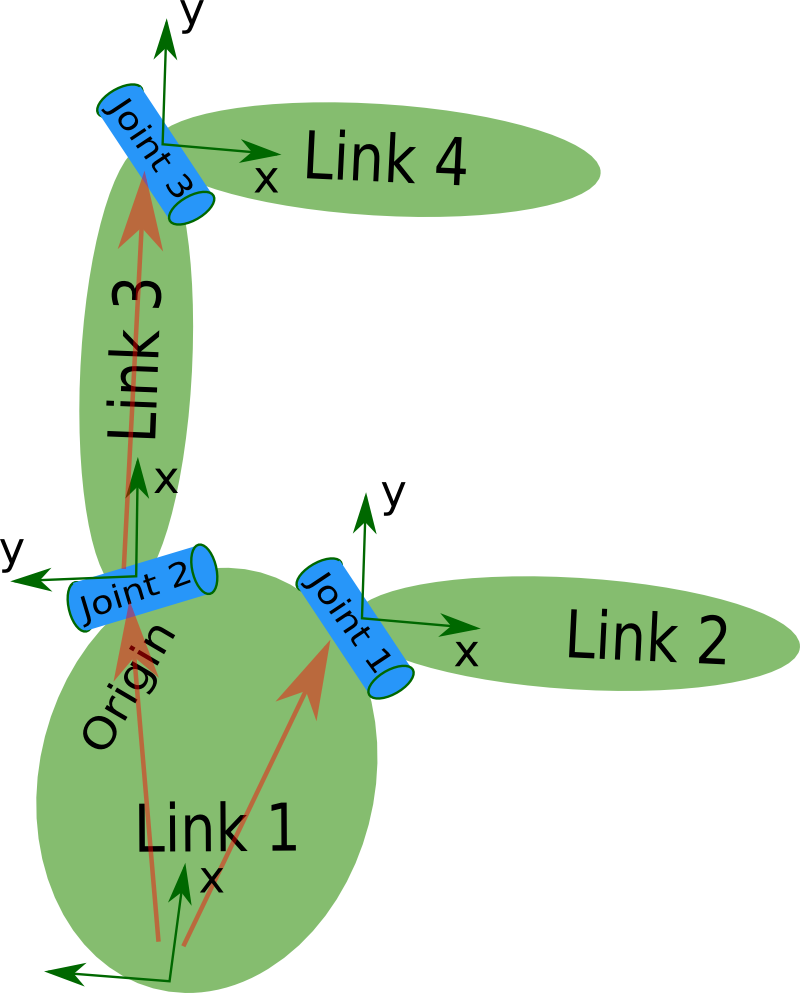
\includegraphics[height=0.3\textwidth]{img/links-joints.png}
% 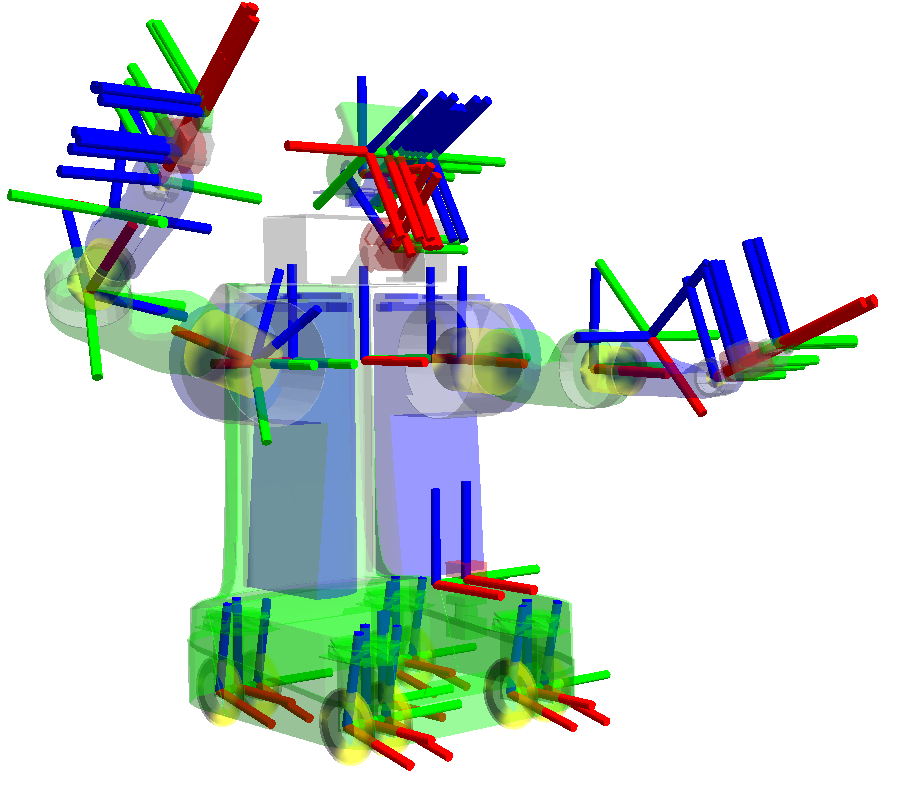
\includegraphics[height=0.3\textwidth]{img/tf-frames.png}
% \end{center}

Pose data is saved in \mongodb collections named ``tf'', the format is described below.

%%%%%%%%%%%%%%%%%%%%%%%%%%%%%%%%%
%%%%%%%%%%%%%%%%%%%%%%%%%%%%%%%%%
\paragraph{Format}
The pose data structure has
fields for encoding the translation and rotation of a coordinate frame.
The parent frame and time stamp of pose estimation
are stored in the \emph{header} field of the data structure.
The transform coordinate frame is assigned to the \emph{child\_frame\_id} field. \\

%The data is stored in the DB collection as array. Each array holding pose estimates for distinct frames at the same time stamp. For indexed search, it is important that each array member has the same time stamp. \\

\def\arraystretch{1.1}%
\begin{figure}[htb]
\begin{center}\begin{tabular}{ >{\ttfamily}p{3.5cm} >{\ttfamily}p{2cm} p{5cm} }
\toprule
\bf Field   & \bf Type & \bf Description \\ \midrule
tf			& dict	& -- \\
\ \ header		& dict		& -- \\
\ \ \ \ seq		& uint32	& consecutively increasing ID \\
\ \ \ \ stamp		& time		& time stamp of this transform \\
\ \ \ \ frame\_id	& string	& parent coordinate frame of this transform \\
\ \ child\_frame\_id	& string	& coordinate frame of this transform \\
\ \ transform		& dict		& -- \\
\ \ \ \ translation	& dict		& -- \\
\ \ \ \ \ \ x		& float64	& \emph{x} axis translation \\
\ \ \ \ \ \ y		& float64	& \emph{y} axis translation \\
\ \ \ \ \ \ z		& float64	& \emph{z} axis translation \\
\ \ \ \ rotation	& dict		& -- \\
\ \ \ \ \ \ x		& float64	& \emph{x} component of quaternion \\
\ \ \ \ \ \ y		& float64	& \emph{y} component of quaternion \\
\ \ \ \ \ \ z		& float64	& \emph{z} component of quaternion \\
\ \ \ \ \ \ w		& float64	& \emph{w} component of quaternion \\
\bottomrule
\end{tabular}\end{center}
\caption{The pose data structure in the \ease system.}
\label{fig:pose_data}
\end{figure}

Note that static frames may be recorded at lower frequency --
about every two seconds.
This usually reduces the data size significantly.
At the moment, no other motion data compression,
such as motion JPEG, is supported.

% From ``Compression of Motion Capture Databases'' Okan Arikan
% The biggest goal of compression is creating a compressed rep-
% resentation of motion that is perceptually as close to the original
% motion as possible. As we will explore later in this paper, a small
% numerical error does not necessarily correspond to a perceptually
% close motion. We would like compression and decompression to be
% as quick as possible. In practice motion capture databases can be
% very big. Therefore another goal for compression and decompres-
% sion is to be able to process without holding the entire database in
% the memory, which may not be possible. Depending on the appli-
% cation we may want to “stream” the data so that the decompressor
% can decode incrementally. We may also want to be able to decode a
% piece of the database without having to decompress any other mo-
% tion

